\documentclass[12pt]{article}
\usepackage[utf8]{inputenc}
\usepackage{geometry}
\geometry{letterpaper, margin=0.25in}
\usepackage{graphicx} 
\usepackage{parskip}
\usepackage{booktabs}
\usepackage{array} 
\usepackage{paralist} 
\usepackage{verbatim}
\usepackage{subfig}
\usepackage{fancyhdr}
\usepackage{sectsty}
\usepackage[shortlabels]{enumitem}

\pagestyle{fancy}
\renewcommand{\headrulewidth}{0pt} 
\lhead{}\chead{}\rhead{}
\lfoot{}\cfoot{\thepage}\rfoot{}

%%% ToC (table of contents) APPEARANCE
\usepackage[nottoc,notlof,notlot]{tocbibind} 
\usepackage[titles,subfigure]{tocloft}
\renewcommand{\cftsecfont}{\rmfamily\mdseries\upshape}
\renewcommand{\cftsecpagefont}{\rmfamily\mdseries\upshape} %

\usepackage{amsmath}
\usepackage{amssymb}
\usepackage{mathtools}
\usepackage{empheq}
\usepackage{xcolor}
\usepackage{bbm}
\usepackage{tikz}
\usepackage{pgfplots}
\usepackage{tikz-cd}
\pgfplotsset{compat=1.18}

\newcommand{\ans}[1]{\boxed{\text{#1}}}
\newcommand{\vecs}[1]{\langle #1\rangle}
\renewcommand{\hat}[1]{\widehat{#1}}

\renewcommand{\P}{\mathbb{P}}
\newcommand{\R}{\mathbb{R}}
\newcommand{\E}{\mathbb{E}}
\newcommand{\Z}{\mathbb{Z}}
\newcommand{\N}{\mathbb{N}}
\newcommand{\Q}{\mathbb{Q}}
\newcommand{\C}{\mathbb{C}}

\newcommand{\ind}{\mathbbm{1}}
\newcommand{\qed}{\quad \blacksquare}

\newcommand{\brak}[1]{\left\langle #1 \right\rangle}
\newcommand{\bra}[1]{\left\langle #1 \right\vert}
\newcommand{\ket}[1]{\left\vert #1 \right\rangle}

\newcommand{\abs}[1]{\left\vert #1 \right\vert}
\newcommand{\mfX}{\mathfrak{X}}
\newcommand{\ep}{\varepsilon}

\newcommand{\Ec}{\mathcal{E}}
\newcommand{\A}{\mathcal{A}}
\newcommand{\F}{\mathcal{F}}
\newcommand{\Cc}{\mathcal{C}}
\newcommand{\B}{\mathcal{B}}
\newcommand{\M}{\mathcal{M}}
\newcommand{\X}{\chi}
\renewcommand{\L}{\mathcal{L}}

\newcommand{\sub}{\subseteq}
\newcommand{\st}{\text{ s.t. }}
\newcommand{\card}{\text{card }}
\renewcommand{\div}{\vspace*{10pt}\hrule\vspace*{10pt}}
\newcommand{\surj}{\twoheadrightarrow}
\newcommand{\inj}{\hookrightarrow}
\newcommand{\biject}{\hookrightarrow \hspace{-8pt} \rightarrow}
\renewcommand{\bar}[1]{\overline{#1}}
\newcommand{\overcirc}[1]{\overset{\circ}{#1}}
\newcommand{\diam}{\text{diam }}

\renewcommand{\Re}{\text{Re}\,}
\renewcommand{\Im}{\text{Im}\,}
\newcommand{\sign}{\text{sign}\,}

\newcommand*{\tbf}[1]{\ifmmode\mathbf{#1}\else\textbf{#1}\fi}

\usepackage{tcolorbox}
\tcbuselibrary{breakable, skins}
\tcbset{enhanced}
\newenvironment*{tbox}[2][gray]{
    \begin{tcolorbox}[
        parbox=false,
        colback=#1!5!white,
        colframe=#1!75!black,
        breakable,
        title={#2}
    ]}
    {\end{tcolorbox}}

\newenvironment*{exercise}[1][red]{
    \begin{tcolorbox}[
        parbox=false,
        colback=#1!5!white,
        colframe=#1!75!black,
        breakable
    ]}
    {\end{tcolorbox}}

\newenvironment*{proof}[1][blue]{
\begin{tcolorbox}[
    parbox=false,
    colback=#1!5!white,
    colframe=#1!75!black,
    breakable
]}
{\end{tcolorbox}}


\title{APMA 1360: Applied Dynamical Systems}
\author{Milan Capoor}
\date{Spring 2025}

\begin{document}
\maketitle

\section{Jan 22}
\subsection*{Motivations - Applications + Phenomena}
\begin{enumerate}
    \item \tbf{Bifurcation theory:} How do systems change as parameters change?

          \emph{Examples:}
          \begin{itemize}
              \item Mechanical systems (e.g. what will happen to a bead as an apparatus is rotated at velocity $\omega$?)
              \item Chemical reactions (e.g. Belusov-Zhabotinsky reaction - oscillations in chemical reactions)
              \item Tipping points (e.g. climate change, convection currents)
              \item Population dynamics (e.g. predator-prey models, outbreaks)
              \item Synchronization (e.g. firefly synchronous lighting, brain activity patterns)
              \item Chaotic dynamics (e.g. double pendulum)
          \end{itemize}

    \item \tbf{Existence and Uniqueness}

    \item \tbf{Dynamical theory}

    \item \tbf{Chaotic dynamics}
\end{enumerate}

\subsection*{Bifurcation Theory}
\tbf{Example (Overdamped bead on loop)}

\begin{center}
    \begin{tikzpicture}
        \draw (0,0) circle (2);

        \node (B) at ({-sqrt(2)},{-sqrt(2)}) {};
        \draw[fill, blue] (B) circle (0.1);

        \draw[dashed, blue] (0,0) -- (B) node[midway, left] {$r$};

        \draw (0, 3) -- (0, -3);
        \draw[->, green!60!black] (0, -1) arc (-90:-130:1) node[midway, below] {$\phi$};

        \draw[->, dashed, red, rotate=-90] ([shift=(-150:0.5)]-2, 0) arc (-150:150:0.1 and 0.5);

    \end{tikzpicture}
\end{center}

\tbf{Goal:} What will happen to the bead as the loop is rotated at velocity $\omega$?

We assume that the only forces on the bead are gravitation, friction, and centrifugal force.

This gives a force diagram:
\begin{center}
    \begin{tikzpicture}

        \draw (0,0) circle (0.05);
        \draw[->] (0, 0) -- (0,-2) node[below] {$mg$};

        \draw (0, 0) arc[start angle =-45, end angle = 0, radius = 2];
        \draw (0, 0) arc[start angle =-45, end angle = -90, radius = 2];

        \draw[->, dashed] (-2,0) -- (0,0);
        \draw[->] (0, 0) -- (2, 0) node[right] {$mr\omega^2\sin \phi$};

        \draw[blue] (-2, -2) -- (2, 2) node[above, right] {Tangent to loop};

        \draw[green!60!black] (0.5, 0)  arc[start angle = 0, end angle = 45, radius = 0.5] node[right] {$\phi$};
    \end{tikzpicture}
\end{center}

From Newton's law,
\[\underbrace{mr \frac{d^2\phi}{dt^2}}_{\text{acceleration}} = -b \frac{d\phi}{dt} - mg \sin \phi + m\omega^2 r \sin\phi \cos \phi\]

Assuming $b \gg 1$, we can neglec
t the LHS so
\begin{align*}
    \frac{d\phi}{dt} & = -\frac{mg}{b}\sin \phi + \frac{m\omega^2 r}{b} \sin \phi \cos \phi    \\
                     & = \frac{mg}{b} \sin \phi \left(\frac{\omega^2 r}{g} \cos \phi- 1\right) \\
                     & = a \sin \phi (\mu \cos \phi - 1)
\end{align*}

\section{Jan 24}
\subsection*{Review}
\tbf{Definition:} A function $u(t)$ is a solution of $\dot u = f(u)$ if $\frac{du(t)}{dt} = f(u(t))$ for all $t$ in some open interval. In this case, we say ``$u(t)$ satisfies $\dot u = f(u)$''.

\begin{tbox}{\textbf{Theorem (Existence and Uniqueness):} Assume $f \in C^1$ (class of continuously differentiable functions) and $u_0 \in \R$ is given. Then the differential equation $\dot u = f(u)$ with initial condition $u(0) = u_0$ has a unique solution $u(t)$ on some open interval containing $t = 0$.}
    \emph{Proof:} Omitted
\end{tbox}

\tbf{Example:} $\dot u = au, u(0) = u_0$ has solution $u(t) = u_0 e^{at}$. Since $au$ is continuous, $u(t) \in C^1$, hence the solution is unique.

\subsection*{Geometric Viewpoint}

\tbf{Example:} Consider $\dot u = f(u)$,
\begin{center}
    \begin{tikzpicture}
        \begin{axis}[
                axis lines=middle,
                no markers,
                enlargelimits,
                xtick=\empty,
                ytick=\empty,
                axis line style={->},
                xlabel style={at={(current axis.right of origin)}, anchor=west},
                ylabel style={at={(current axis.above origin)}, anchor=south},
                domain=-6:6,
                samples=20
            ]
            \addplot[blue, thick] {-(x+5)*(2*x+3)*(x-5)};

            \node[red, above] (u1) at (axis cs:-5,-0.6) {$u_1$};
            \node[red, above] (u2) at (axis cs:-3/2,0) {$u_2$};
            \node[red, right, above] (u3) at (axis cs:5,0) {$u_3$};

            \coordinate (u1) at (axis cs:-5,0);
            \coordinate (u2) at (axis cs:-3/2,0);
            \coordinate (u3) at (axis cs:5,0);

        \end{axis}
        \draw[red, fill] (u1) circle (0.05);
        \draw[red, fill] (u2) circle (0.05);
        \draw[red, fill] (u3) circle (0.05);

    \end{tikzpicture}
\end{center}

For each point, $f(u_i) = 0 \implies u(t) = u_i$ is a solution for all $t$.

We can check:
\[\begin{cases}
        \frac{du}{dt}(t) = \frac{d}{dt} u_i = 0 \\
        f(u(t)) = f(u_i) = 0
    \end{cases}\]
Hence, $u(t) = u_i$ is a solution.

We call the points $u_1, u_2, u_3$ \emph{equilibrium points}, \emph{rest states}, \emph{steady states}, \emph{fixed points}, or \emph{stationary points}.

We can also consider the direction field of $\dot u = f(u(t))$:
\[\begin{cases}
        f(u) < 0 \implies u \text{ decreasing} \implies u \text{ moves left} \\
        f(u) > 0 \implies u \text{ increasing} \implies u \text{ moves right}
    \end{cases}\]

So we can draw the phase diagram
\begin{center}
    \begin{tikzpicture}
        \begin{axis}[
                axis lines=middle,
                no markers,
                enlargelimits,
                xtick=\empty,
                ytick=\empty,
                axis line style={->},
                xlabel style={at={(current axis.right of origin)}, anchor=west},
                ylabel style={at={(current axis.above origin)}, anchor=south},
                domain=-6:6,
                samples=20
            ]
            \addplot[blue, thick] {-(x+5)*(2*x+3)*(x-5)};

            \node[red, above] (u1) at (axis cs:-5, 0) {$u_1$};
            \node[red, above] (u2) at (axis cs:-3/2,0) {$u_2$};
            \node[red, above] (u3) at (axis cs:5,0) {$u_3$};

            \coordinate (u1) at (axis cs:-5,0);
            \coordinate (u2) at (axis cs:-3/2,0);
            \coordinate (u3) at (axis cs:5,0);


            \node[green!60!black] at (axis cs:-4.5, 0) {$<$};
            \node[green!60!black] at (axis cs:-5.5, 0) {$>$};

            \node[green!60!black] at (axis cs:-2, 0) {$<$};
            \node[green!60!black] at (axis cs:-1, 0) {$>$};

            \node[green!60!black] at (axis cs:4.5, 0) {$>$};
            \node[green!60!black] at (axis cs:5.5, 0) {$<$};
        \end{axis}
        \draw[red, fill] (u1) circle (0.05);
        \draw[red, fill] (u2) circle (0.05);
        \draw[red, fill] (u3) circle (0.05);


    \end{tikzpicture}
\end{center}

In this case, we say that $u_1, u_3$ are stable but $u_2$ is unstable.

\tbf{Stable:} an equilibrium $u_i$ is stable if all solutions for initial conditions near $u_i$ converge to $u_i$ as $t \to \infty$.

\tbf{Unstable:} an equilibrium $u_i$ is unstable if there exists an initial condition near (but distinct from) $u_i$ such that the solution moves away from $u_i$ as $t \to \infty$.

\tbf{Conditions for stability:} Assuming $u_i$ is an equilibrium,
\begin{itemize}
    \item If $f'(u_i) < 0$, then $u_i$ is stable.
    \item If $f'(u_i) > 0$, then $u_i$ is unstable.
    \item If $f'(u_i) = 0$, then it is undetermined
\end{itemize}

What can $f'(u_i) = 0$ look like?

\emph{Examples:}

\begin{center}
    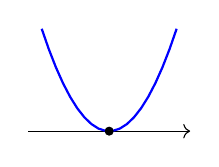
\begin{tikzpicture}
        \begin{axis}[
                width=0.3\textwidth,
                axis lines=middle,
                no markers,
                enlargelimits,
                xtick=\empty,
                ytick=\empty,
                axis line style={->},
                domain=-2:2,
                samples=20,
                hide y axis
            ]
            \addplot[blue, thick] {x^2};
            \coordinate (O) at (axis cs: 0, 0);
        \end{axis}
        \draw[fill] (O) circle (0.05);
    \end{tikzpicture}
    \hspace{1cm}
    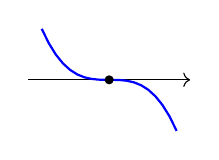
\begin{tikzpicture}
        \begin{axis}[
                width=0.3\textwidth,
                axis lines=middle,
                no markers,
                enlargelimits,
                xtick=\empty,
                ytick=\empty,
                axis line style={->},
                domain=-2:2,
                samples=20,
                hide y axis
            ]
            \addplot[blue, thick] {-x^3};
            \coordinate (O) at (axis cs: 0, 0);
        \end{axis}
        \draw[fill] (O) circle (0.05);

    \end{tikzpicture}
\end{center}

\subsection*{Example 1 Revisited:} Recall
\[\dot \phi = a \sin \phi(\mu \cos \phi - 1) = f(\phi)\]
for $a, \mu > 0$ and $\mu \approx \omega^2$.

\begin{enumerate}
    \item We can verify $f \in C^1$.

    \item Find the equilibrium points:
          \[a \sin \phi (\mu \cos \phi - 1) = 0 \implies \phi = \{0, \pi\}\]

    \item Determine stability:
          \begin{align*}
              f'(\phi) \bigg\vert_{\phi = 0, \pi} & = \left[a \cos \phi (\mu \cos \phi - 1)\right]_{\phi = 0, \pi} \\
                                                  & = \begin{cases}
                                                          a(\mu - 1) & \phi = 0   \\
                                                          a(\mu + 1) & \phi = \pi
                                                      \end{cases}
          \end{align*}

          Hence, $\phi = 0$ is always unstable since $a(\mu + 1) > 0$. $\phi = \pi$ is stable $\mu < 1$, unstable $\mu > 1$ and undetermined for $\mu = 1$.

          In fact, this makes sense. $\mu$ is the ratio of the centrifugal force to the gravitational force. If $\mu < 1$, the gravitational force is stronger and the bead will fall to the bottom. If $\mu > 1$, the centrifugal force is stronger and the bead will move outwards.

\end{enumerate}


\section{Jan 27}
\tbf{Recall:} We return one more time to the example of the bead on a loop. Last time, we determined the system has equilibria
\begin{center}
    %% Bead on loop equilibrium diagram
    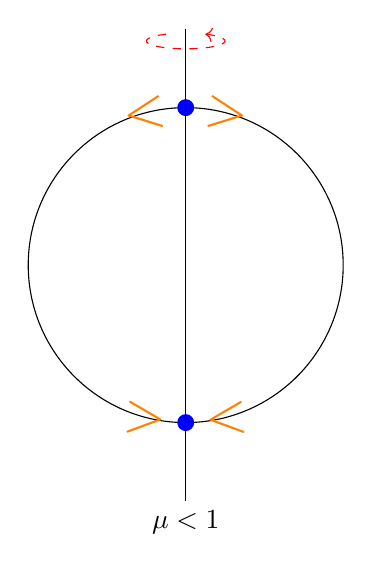
\begin{tikzpicture}
        \draw (0,0) circle (2);

        \node (top) at (0, 2) {};
        \node (bot) at (0, -2) {};
        \draw[fill, blue] (top) circle (0.1);
        \draw[fill, blue] (bot) circle (0.1);

        \node[scale=2, orange, rotate=-8] at (top) [right] {$>$};
        \node[scale=2, orange, rotate=8] at (top) [left] {$<$};

        \node[scale=2, orange, rotate=5] at (bot) [right] {$<$};
        \node[scale=2, orange, rotate=-5] at (bot) [left] {$>$};


        \draw (0, 3) -- (0, -3) node[below] {$\mu < 1$};

        \draw[->, dashed, red, rotate=-90] ([shift=(-150:0.5)]-2.5, 0) arc (-150:150:0.1 and 0.5);
    \end{tikzpicture}
    \hspace{1cm}
    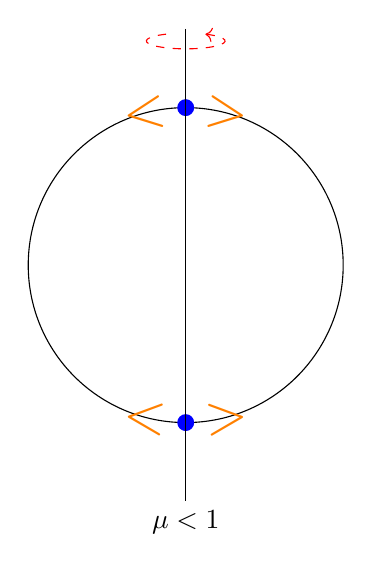
\begin{tikzpicture}
        \draw (0,0) circle (2);

        \node (top) at (0, 2) {};
        \node (bot) at (0, -2) {};
        \draw[fill, blue] (top) circle (0.1);
        \draw[fill, blue] (bot) circle (0.1);

        \node[scale=2, orange, rotate=-8] at (top) [right] {$>$};
        \node[scale=2, orange, rotate=8] at (top) [left] {$<$};

        \node[scale=2, orange, rotate=5] at (bot) [right] {$>$};
        \node[scale=2, orange, rotate=-5] at (bot) [left] {$<$};


        \draw (0, 3) -- (0, -3) node[below] {$\mu < 1$};

        \draw[->, dashed, red, rotate=-90] ([shift=(-150:0.5)]-2.5, 0) arc (-150:150:0.1 and 0.5);



    \end{tikzpicture}
\end{center}

In the case on the right, the equilibria are not consistent. Therefore, there need to be additional equilibria.

We can check:
\[f(\phi) - a \sin \phi (\mu \cos \phi - 1)\]

Setting $a \sin \phi = 0$ gives $\phi = \{0, \pi\}$. Taking $\mu \cos \phi - 1 = 0$ gives $\phi = \arccos \frac{1}{\mu}$:
\begin{center}
    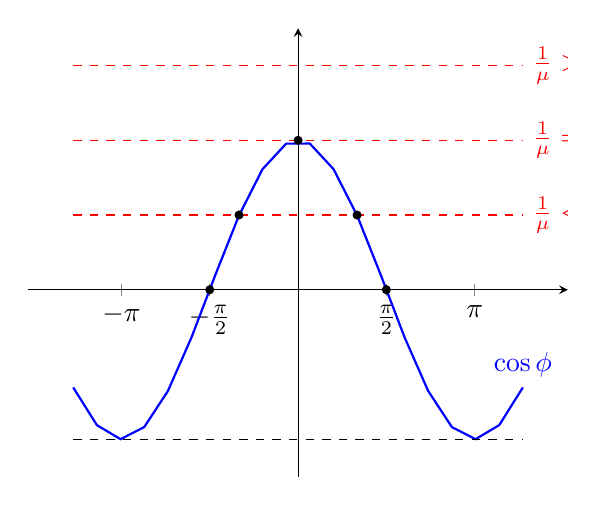
\begin{tikzpicture}
        \begin{axis}[
                axis lines=middle,
                no markers,
                enlargelimits,
                xtick={-pi, -pi/2, 0, pi/2, pi},
                ytick=\empty,
                xlabel=\empty,
                xticklabels={$-\pi$, $-\frac{\pi}{2}$, 0, $\frac{\pi}{2}$, $\pi$},
                domain=-4:4,
                samples=20
            ]
            \addplot[blue, thick] {cos(deg(x))};
            \addplot[red, dashed] {3/2} node[right] {$\frac{1}{\mu}> 1$};
            \addplot[red, dashed] {1} node[right] {$\frac{1}{\mu} = 1$};
            \addplot[red, dashed] {1/2} node[right] {$\frac{1}{\mu}< 1$};
            \addplot[dashed] {-1};


            \coordinate (A) at (axis cs: pi/2, 0);
            \coordinate (B) at (axis cs: -pi/2, 0);
            \coordinate (C) at (axis cs: 0, 1);
            \coordinate (D) at (axis cs: 1.05, 1/2);
            \coordinate (E) at (axis cs: -1.05, 1/2);

            \coordinate (lab) at (axis cs: 4, -0.5);


        \end{axis}
        \draw[fill] (A) circle (0.05);
        \draw[fill] (B) circle (0.05);
        \draw[fill] (C) circle (0.05);
        \draw[fill] (D) circle (0.05);
        \draw[fill] (E) circle (0.05);

        \node[blue] at (lab) {$\cos \phi$};



    \end{tikzpicture}
\end{center}

This gives us the bifurcation diagram:

\begin{center}
    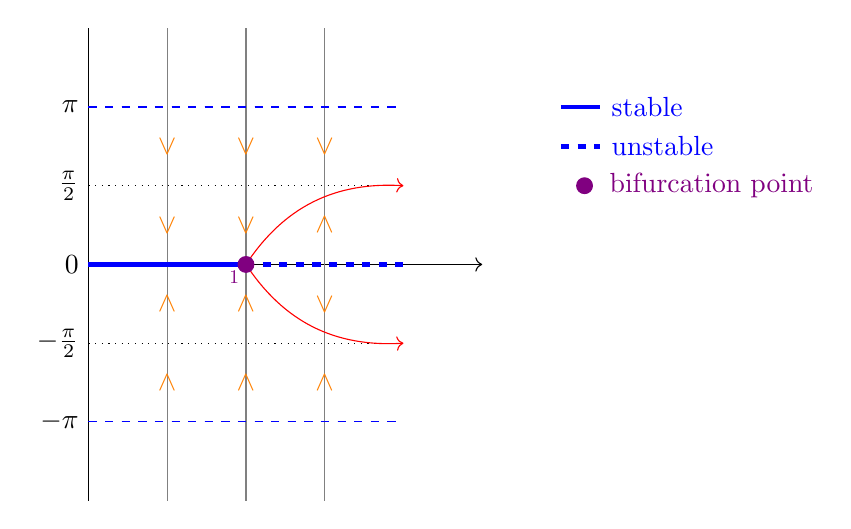
\begin{tikzpicture}
        \node[left] (O) at (0, 0) {$0$};
        \draw (0, -3) -- (0, 3); % y-axis
        \draw[->] (0, 0) -- (5, 0); % x-axis

        \node[left] (pi-y) at (0, 2) {$\pi$};
        \draw[dashed, blue] (pi-y) -- (4, 2);
        \node[left] (pi2-y) at (0, 1) {$\frac{\pi}{2}$};
        \draw[dotted] (pi2-y) -- (4, 1);

        \node[left] (mpi-y) at (0, -2) {$-\pi$};
        \draw[dashed, blue] (mpi-y) -- (4, -2);
        \node[left] (mpi2-y) at (0, -1) {$-\frac{\pi}{2}$};
        \draw[dotted] (mpi2-y) -- (4, -1);

        \draw[gray] (1, -3) -- (1, 3);
        \draw[gray] (2, -3) -- (2, 3);
        \draw[gray] (3, -3) -- (3, 3);

        \draw[blue, ultra thick] (0, 0) -- (2, 0);
        \draw[blue, ultra thick, dashed] (2, 0) -- (4, 0);
        \draw[blue, dashed] (0,2) -- (4, 2);
        \draw[blue, dashed] (0,-2) -- (4, -2);

        \node[orange] at (1, 1.5) {\rotatebox{180}{$\wedge$}};
        \node[orange] at (2, 1.5) {\rotatebox{180}{$\wedge$}};
        \node[orange] at (3, 1.5) {\rotatebox{180}{$\wedge$}};
        \node[orange] at (1, 0.5) {\rotatebox{180}{$\wedge$}};
        \node[orange] at (2, 0.5) {\rotatebox{180}{$\wedge$}};
        \node[orange] at (3, 0.5) {$\wedge$};

        \node[orange] at (1, -0.5) {$\wedge$};
        \node[orange] at (2, -0.5) {$\wedge$};
        \node[orange] at (3, -0.5) {\rotatebox{180}{$\wedge$}};
        \node[orange] at (1, -1.5) {$\wedge$};
        \node[orange] at (2, -1.5) {$\wedge$};
        \node[orange] at (3, -1.5) {$\wedge$};

        \draw[->, red] (2, 0) to[bend left] (4, 1);
        \draw[->, red] (2, 0) to[bend right] (4, -1);

        \draw[red!50!blue, fill] (2, 0) circle (0.1) node[scale=0.7, below left]{$1$};

        \draw[blue, ultra thick] (6, 2) -- (6.5, 2) node[right] {stable};
        \draw[blue, ultra thick, dashed] (6, 1.5) -- (6.5, 1.5) node[right] {unstable};
        \draw[red!50!blue, fill] (6.3, 1) circle (0.1) node[right]{\;\;bifurcation point};


    \end{tikzpicture}
\end{center}




where the curve is given by $\mu = \frac{r\omega^2}{g} \approx \frac{\text{centrifugal}}{\text{gravitational}}$.

Notice if $f'(\phi_*) \neq 0$, then the equilibrium $\phi_*$ varies continuously with $\mu$. If $f'(\phi_*) =0$, then new equilibria emerge and dynamics change.

\subsection*{Parameter-Dependent Differential Equations:} Consider $\dot u = f(u, \mu)$ for $u, \mu \in \R$ and $f: \R^2 \to \R$.

\tbf{Example:} $f(u, 0) = u$
%% $f(u, 0) = u$.
\begin{center}
    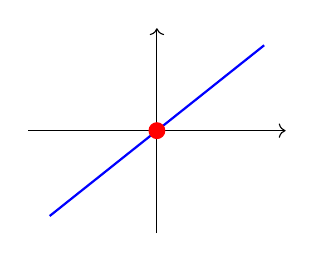
\begin{tikzpicture}
        \begin{axis}[
                width=0.4\textwidth,
                axis lines=middle,
                no markers,
                enlargelimits,
                xtick=\empty,
                ytick=\empty,
                axis line style={->},
                domain=-1:1,
                samples=20,
            ]
            \addplot[blue, thick] {x};
            \coordinate (O) at (axis cs: 0, 0);
        \end{axis}
        \draw[fill, red] (O) circle (0.1        );
    \end{tikzpicture}
\end{center}

Here, $u = 0$ is an unstable equilibrium. ($f(0, 0) =0$ and $f_u(0, 0) = 1 > 0$).

What happens if we change $\mu$ slightly? Choose $\mu \approx 0$:

\begin{center}
    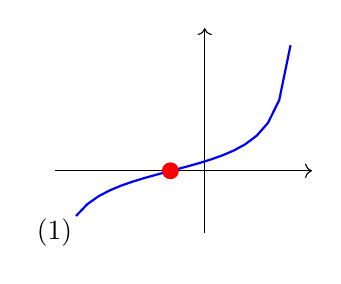
\begin{tikzpicture}
        \begin{axis}[
                width=0.4\textwidth,
                axis lines=middle,
                no markers,
                enlargelimits,
                xtick=\empty,
                ytick=\empty,
                axis line style={->},
                domain=-1.5:1,
                samples=20,
            ]
            \addplot[blue, thick] {tan(deg(x+pi/8))};
            \coordinate (O) at (axis cs: -0.4, 0);
        \end{axis}
        \draw[fill, red] (O) circle (0.1);
        \node (0, 0) {(1)};
    \end{tikzpicture}
    \hspace{1cm}
    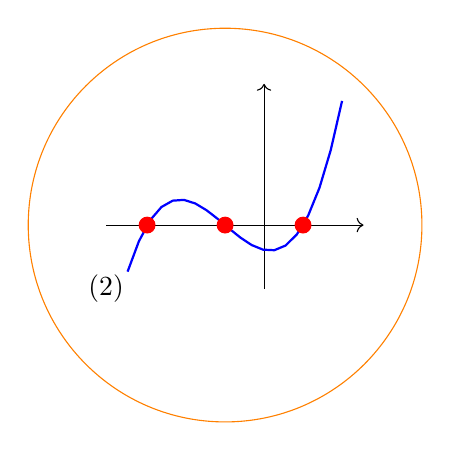
\begin{tikzpicture}
        \begin{axis}[
                width=0.4\textwidth,
                axis lines=middle,
                no markers,
                enlargelimits,
                xtick=\empty,
                ytick=\empty,
                axis line style={->},
                domain=-3.5:2,
                samples=20,
            ]
            \addplot[blue, thick] {(x+3)*(x+1)*(x-1)};
            \coordinate (A) at (axis cs: -3, 0);
            \coordinate (B) at (axis cs: -1, 0);
            \coordinate (C) at (axis cs: 1, 0);

            \coordinate (O) at (axis cs: -1, 0);

        \end{axis}
        \draw[fill, red] (A) circle (0.1);
        \draw[fill, red] (B) circle (0.1);
        \draw[fill, red] (C) circle (0.1);

        \draw[orange] (O) circle (2.5);


        \node (0, 0) {(2)};
    \end{tikzpicture}
\end{center}

On the left, the equilibrium moves but is unique and still unstable. On the right, we have three equilibria and we can shrink the ball as $\mu \to 0$.

For (2), say
\[f(u, \mu) = \begin{cases}
        u + \mu                            & u \leq -\mu          \\
        \frac{u}{2}(\frac{u^2}{\mu^2} - 1) & -\mu \leq u \leq \mu \\
        u - \mu                            & u = \mu
    \end{cases}\]
with $\abs{f(u, \mu)} \leq \text{const.}$ uniformly in $\mu, u$

\tbf{Properties of (2):}
\begin{itemize}
    \item $f(u, \mu)$ is continuous in $u, \mu$.
    \item $f(u, \mu)$ is differentiable in $u$ for all $(u, \mu)$
    \item $f_u(u, \mu)$ is not continuous
\end{itemize}

For simplicity, we will consider only functions $f(u, \mu)$ that are infinitely often differentiable and for which all derivatives are continuous in $(u, \mu)$, i.e. $f \in C^{\infty}(\R^2, \R) = C^{\infty}$

\tbf{Goal:} Assume $u_0$ is an equilibrium $\dot u = f(u, \mu)$ for $\mu = \mu_0$ so that when $f_u(u_0, \mu_0) \neq 0$, there is a function $g(\mu)$ so that $f(u, \mu) = 0$ for $(u, \mu)$ near $(u_0, \mu_0)$ iff $u = g(\mu)$.

\begin{center}
    \begin{tikzpicture}
        % Draw the axes
        \draw[->] (0,0) -- (5,0) node[right] {$\mu$};
        \draw[->] (0,0) -- (0,5) node[above] {$u$};

        % Draw the tick and label at the center
        \draw (0.2,2.5) -- (-0.3,2.5) node[left] {$u_0$};
        \draw (2.5,0.2) -- (2.5,-0.3) node[below] {$\mu_0$};
        \node[below right] at (2.5,2.5) {$(\mu_0, u_0)$};

        \draw[fill] (2.5, 2.5) circle (0.05);

        % Draw the curve
        \draw[blue, thick, domain=0:5, samples=20] plot (\x, {2.5 + 2.5*sin((\x-2.5)*180/5)}) node[right] {$\{(u, \mu): f(u, \mu) = 0\}$};

    \end{tikzpicture}
\end{center}

\begin{tbox}{\textbf{Implicit Function Theorem}: Assume $f(u_0, \mu_0) = 0$ and $f_u(u_0, \mu_0)\neq 0$ for $f \in C^{\infty}$. Then there exists open  intervals, $I, J$ with $u_0 \in J, \mu_0 \in I$ and a $g: I \to J$ such that $f(u, \mu) = 0$ for $(u, \mu) \in J \times I$ iff $u =g(\mu)$. Furthermore, $g \in C^{\infty}$. In particular, if $u_0$ is an equilibrium of $\dot u = f(u, \mu)$ at $\mu = \mu_0$ with $f_u(u_0, \mu_0) \neq 0$, then $\dot u = f(u, \mu)$ has an equilibrium in $J  \times I$ iff $u = g(\mu)$ and these equilibria share their stability properties with $u_0$}
    \emph{Example:}
    \begin{center}
        \begin{tikzpicture}
            % Draw the axes
            \draw[->] (0,0) -- (5,0) node[right] {$\mu$};
            \draw[->] (0,0) -- (0,5) node[above] {$u$};

            % Draw the tick and label at the center
            \draw (0.2,2.5) -- (-0.3,2.5) node[red, left] {$u_0$};
            \draw (2.5,0.2) -- (2.5,-0.3) node[red, below] {$\mu_0$};

            \draw[red, fill] (2.5, 2.5) circle (0.1);

            % Draw the curve
            \draw[blue, thick, domain=0:5, samples=20] plot (\x, {2.5 + 2.5*sin((\x-2.5)*180/5)}) node[right] {$u=g(\mu)$};

            \draw[orange!90!black, ultra thick] (2, 0) -- (3, 0) node[below right] {$I$};
            \draw[orange!90!black, ultra thick] (0, 2) -- (0, 3) node[above left] {$J$};

            \draw[orange, dashed, ultra thick] (2, 2) -- (3, 2) -- (3, 3) -- (2, 3) -- cycle;

        \end{tikzpicture}
    \end{center}
    \div
    \emph{Proof:} Omitted
\end{tbox}

\section{Jan 29}
\subsection{Implicit Function Theorem}re
\tbf{Recall:} If we have $f = f(u, \mu) \in C^{\infty}$ with $f(u_0, \mu_0) = 0$ and $f_u(u_0, \mu_0) \neq 0$, then there exist open intervals $I, J$ with $\mu_0 \in I$, $u_0 \in J$ and a unique $g: I \to J$ with $g(\mu_0) = u_0$ so that $f(u, \mu) = 0$ for $(u, \mu) \in J \times I$ iff $u = g(\mu)$. Furthermore, $g \in C^{\infty}$.

\begin{center}
    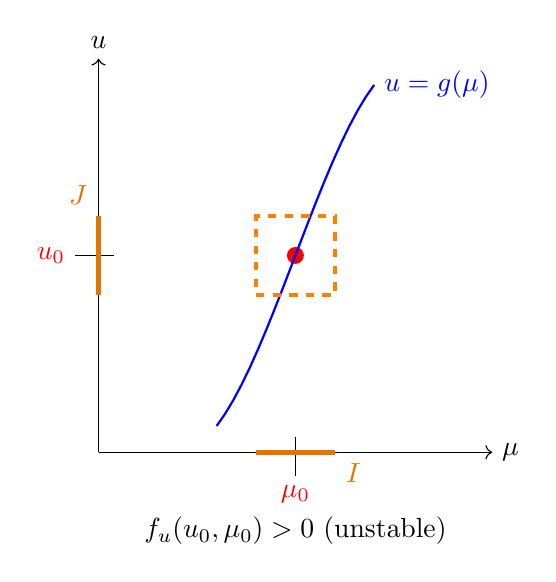
\begin{tikzpicture}
        % Draw the axes
        \draw[->] (0,0) -- (5,0) node[right] {$\mu$};
        \draw[->] (0,0) -- (0,5) node[above] {$u$};

        % Draw the tick and label at the center
        \draw (0.2,2.5) -- (-0.3,2.5) node[red, left] {$u_0$};
        \draw (2.5,0.2) -- (2.5,-0.3) node[red, below] {$\mu_0$};

        \draw[red, fill] (2.5, 2.5) circle (0.1);

        % Draw the curve
        \draw[blue, thick, domain=1.5:3.5, samples=20] plot (\x, {2.5 + 2.5*sin((\x-2.5)*180/3)}) node[right] {$u=g(\mu)$};

        \draw[orange!90!black, ultra thick] (2, 0) -- (3, 0) node[below right] {$I$};
        \draw[orange!90!black, ultra thick] (0, 2) -- (0, 3) node[above left] {$J$};

        \draw[orange, dashed, ultra thick] (2, 2) -- (3, 2) -- (3, 3) -- (2, 3) -- cycle;

        \node at (2.5, -1) {$f_u(u_0, \mu_0) > 0 \text{ (unstable)}$};
    \end{tikzpicture}
    \hspace{1cm}
    \begin{tikzpicture}
        % Draw the axes
        \draw[->] (0,0) -- (5,0) node[right] {$\mu$};
        \draw[->] (0,0) -- (0,5) node[above] {$u$};

        % Draw the tick and label at the center
        \draw (0.2,2.5) -- (-0.3,2.5) node[red, left] {$u_0$};
        \draw (2.5,0.2) -- (2.5,-0.3) node[red, below] {$\mu_0$};

        \draw[red, fill] (2.5, 2.5) circle (0.1);

        % Draw the curve
        \draw[blue, thick, domain=1.5:3.5, samples=20] plot (\x, {2.5 + (\x-2.5)^2}) node[right] {$u=g(\mu)$};

        \draw[orange!90!black, ultra thick] (2, 0) -- (3, 0) node[below right] {$I$};
        \draw[orange!90!black, ultra thick] (0, 2) -- (0, 3) node[above left] {$J$};

        \draw[orange, dashed, ultra thick] (2, 2) -- (3, 2) -- (3, 3) -- (2, 3) -- cycle;

        \node at (2.5, -1) {$f_u(u_0, \mu_0) < 0 \text{ (stable)}$};


    \end{tikzpicture}
\end{center}

\tbf{Definition:} we say that $u_0$ is a \tbf{hyperbolic equilibrium} of $\dot u = f(u, \mu)$ at $\mu = \mu_0$ if
\begin{itemize}
    \item $f(u_0, \mu_0) = 0$ ($u_0$ is an equilibrium)
    \item $f_u(u_0, \mu_0) \neq 0$ ($u_0$ is hyperbolic)
\end{itemize}

\emph{Example:} if $u_0$ is \emph{not} hyperbolic, the dynamics can be more complicated when we vary $\mu$ near $\mu_0$.

\begin{center}
    % Right Parabola
    \begin{tikzpicture}
        \draw (0, 0) -- (5, 0) node[right] {$\mu$};
        \draw (0, -2) -- (0, 2) node[above] {$u$};

        \coordinate (pt) at (2.5, 0);
        \begin{axis}[at=(pt), anchor=west, no markers, axis lines=middle, hide y axis, hide x axis]
            \addplot[blue] ({x^2}, x);
        \end{axis}

        \draw[red, ultra thick] (0, 0) -- (2.5, 0);
        \draw[red, ultra thick, dashed] (2.5, 0) -- (5, 0);

        \draw[red, fill] (2.5, 0) circle (0.1) node[below left] {$f_u(0, 1) = 0$};
    \end{tikzpicture}
\end{center}

Here the equilibrium on the red line is hyperbolic.

\tbf{Catalogue of Bifurcations:}
\begin{itemize}
    \item Consider $\dot u = f(u, \mu)$ with $u, \mu \in \R$ and $f \in C^{\infty}$.
    \item Assume WLOG that $(u, \mu) = (0, 0)$ is an equilibrium with
          \[\begin{cases}
                  f(0, 0) = 0 \\
                  f_u(0, 0) = 0
              \end{cases}\]
          (i.e. $(0, 0)$ is not hyperbolic)

    \item \tbf{Goal:} find all equilibria of $\dot u = f(u, \mu)$ near $(0, 0)$ and determine their stability.
\end{itemize}

Since we only need to examine the behavior around $(0, 0)$, we can use a \emph{Taylor Expansion:}

(where $O: \R^2 \to \R$ goes to $0$ at least cubically as $u, \mu \to 0$)

Plugging in our conditions,
\[f(u, \mu) = f_{\mu}(0, 0) \mu + \frac{1}{2}f_{uu}(0,0)u^2 + f_{u\mu}(0, 0)u\mu + \frac{1}{2}f_{\mu\mu}(0, 0)\mu^2 + O({\abs{u}+ \abs{\mu}}^3)\]

From here, we will
\begin{enumerate}
    \item start from terms of lowest order to highest order monomials and assume that coefficients are non-zero.
    \item we already assumed $f(0, 0) = 0$ and $f_u(0, 0) = 0$ so there are no choices left
    \item hence, assume the coefficient $a$ of $f_{\mu}(0, 0)$ is non-zero
\end{enumerate}

Hence,
\[f(u, \mu) = a\mu + O((\abs{u} + \abs{\mu})^2) = 0\]
(where we set it to $0$ as we are looking for equilibria)

Then, by the Implicit Function Theorem, we have a unique function $g$ in a neighborhood of $(0, 0)$ with $g(0) = 0$ and $\mu = g(u)$.

Now we have a few potential cases:
\begin{center}
    % Cubic 
    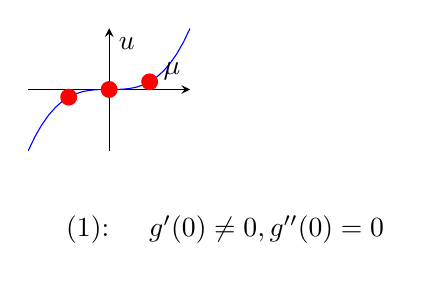
\begin{tikzpicture}
        \begin{axis}
            [
                width=0.3\textwidth,
                axis lines=middle,
                no markers,
                domain=-2:2,
                xtick=\empty,
                ytick=\empty,
                xlabel={$\mu$},
                ylabel={$u$}
            ]
            \addplot[blue] {x^3};
            \coordinate (O) at (axis cs: 0, 0);
            \coordinate (r) at (axis cs: 1, 1);
            \coordinate (l) at (axis cs: -1, -1);
        \end{axis}

        \draw[red, fill] (O) circle (0.1);
        \draw[red, fill] (r) circle (0.1);
        \draw[red, fill] (l) circle (0.1);

        %\draw[blue, thick, domain=0:5, samples=20] plot (\x, {2.5 + 2.5*sin((\x-2.5)*180/5)}) node[right] {$\mu=g(u)$};

        \node at (2.5, -1) {(1): \quad $g'(0)\neq 0, g''(0) = 0$};
    \end{tikzpicture}
    \hspace*{1cm}
    % Left parabola
    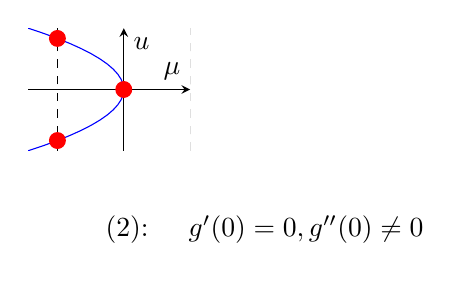
\begin{tikzpicture}
        \begin{axis}[
                width=0.3\textwidth,
                no markers,
                axis lines=middle,
                domain=-1.2:1.2,
                xtick=\empty,
                ytick=\empty,
                xlabel={$\mu$},
                ylabel={$u$}]
            \addplot[blue] ({-x^2}, x);

            \addplot[dashed] ({-1}, x);
            \addplot[dashed] ({1}, x);

            \coordinate (u1) at (axis cs:-1, -1);
            \coordinate (u2) at (axis cs:-1, 1);
            \coordinate (o) at (axis cs:0, 0);
        \end{axis}
        \draw[red, fill] (u1) circle (0.1);
        \draw[red, fill] (u2) circle (0.1);
        \draw[red, fill] (o) circle  (0.1);

        \node at (3, -1) {(2): \quad $g'(0) = 0, g''(0) \neq 0$};
    \end{tikzpicture}
    \hspace{1cm}
    % Line 
    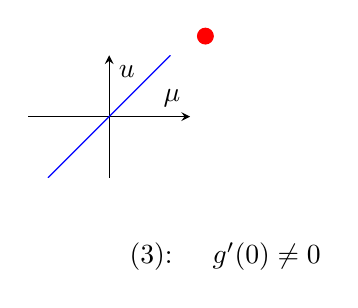
\begin{tikzpicture}
        \begin{axis}[
                width=0.3\textwidth,
                axis equal,
                axis lines=middle,
                no markers,
                xlabel={$\mu$},
                ylabel={$u$},
                xtick=\empty,
                ytick=\empty,
            ]
            \addplot[blue, smooth, domain=-5:5, samples=20] {x};

        \end{axis}

        \draw[red, fill] (2.25, 1.8) circle (0.1);

        \node at (2.5, -1) {(3): \quad $g'(0) \neq0$};
    \end{tikzpicture}

\end{center}

On the left, we gave a unique equilibrium for $\mu$ near $0$. On the right, as $\mu$ increases, two equilibria collide at $\mu =0$ and disappear. Notice that this is different than the case in the logistic model from HW where only one equilibrium disappeared and from the bead on a loop example where two equilibria merged. In some sense, this is a more complicated bifurcation, but also the most common in applications.


\section{Jan 31}
\tbf{Setup:} $u = 0$ is a non-hyperbolic equilibrium at $\mu = 0$, i.e. $f(0, 0) = 0$ and $f_u(0, 0) = 0$.  We want to find solutions of $f = f(u, \mu)$.

Making the assumption, $f_{\mu}(0, 0) = a \neq 0$, we show that $f(u, \mu)=  0$ for $(u, \mu)$ near $(0, 0)$ iff $\mu = g(u)$ with $g(0) = 0$ and $g \in C^{\infty}$.

Formulated differently,we know that $f(u, g(u)) = 0$ for all $u$. Differentiating in $u$, we get
\[0 = \frac{d}{du}(f(u, g(u))) = f_u(u, g(u)) + f_{\mu}(u, g(u))g'(u) \tag{(*)}\]
for all $u$ near $0$

Evaluating at $u = 0$,
\[0 = f_u(0, 0) + f_{\mu}(0, 0)g'(0) = ag'(0) \implies g'(0) = 0\]

From (*), we know that case (1) above is impossible. Can we determine $g''(0)$?

Differentiating again,
\begin{align*}
    0 & = f_u(u, g(u)) + f_{\mu}(u, g(u))g'(u)                                                                                        \\
    0 & = f_{uu}(u, g(u)) + f_{u \mu}(u, g(u))g'(u) + f_{\mu u}(u, g(u)) g'(u) + f_{\mu \mu}(u, g(u))g'(u)^2 + f_{\mu}(u, g(u))g''(u) \\
\end{align*}

Evaluating at $u = 0$,
\begin{align*}
    0 & = f_{uu}(0, 0) + 2f_{u\mu}(0, 0 ) g'(0) + f_{\mu\mu}(0, 0)g''(0)^2 + f_{\mu}(0, 0)g''(0) \\
      & = f_{uu}(0, 0) + f_{\mu}(0, 0)g''(0)
    g''(0) = -\frac{f_{uu}(0, 0)}{f_{\mu}(0, 0)}
\end{align*}

We assume $f_{uu}(0, 0) \neq 0$ to put us in Case (2) above.

\tbf{Remark:} there is no reason we could not have chosen $f_{uu}(0, 0) = 0$ to look at (3). However, in some sense Case (2) is more interesting and also has less tedious calculations. Further, it would be somewhat surprising for there to be neither first nor second derivatives in a Taylor Expansion. In general, though, this choice was arbitrary.

In particular,
\[g(u) = -\frac{1}{2} \frac{f_u(0, 0)}{f_{\mu}(0, 0)} u^2 + O(u^3)\]

\tbf{Conclusion (Existence):} Assume $f(0, 0) = 0, f_u(0, 0) = 0, f_{\mu}(0, 0) \neq 0, f_{uu}(0, 0) \neq 0$. Then $f(u, \mu) = 0$ vanishes near $(0, 0)$ iff $\mu = g(u)$ with $g = -\frac{1}{2} \frac{f_u(0, 0)}{f_{\mu}(0, 0)} u^2 + O(u^3)$.

\subsection{Bifurcation Analysis}

Here, $-\frac{f_u(0, 0)}{f_{\mu}(0, 0)} < 0$ and $\mu < 0$ corresponds to having precisely two rest states, while $\mu > 0$ has none.

The prototypical equation which satisfies our hypothesis is
\[f(u, \mu) = \mu - u^2\]

This gives three possible graphs:

\begin{center}
    \begin{tikzpicture}
        \begin{axis}[
                width=0.3\textwidth,
                axis lines=middle,
                axis equal,
                no markers,
                domain=-1.2:1.2,
                xtick=\empty,
                ytick=\empty]

            \addplot[blue, samples=20] {-x^2} node[below left] {$f(u, 0) = -u^2$};

            \coordinate (O) at (axis cs: 0, 0);
            \coordinate (l) at (axis cs: -0.5, 0);
            \coordinate (r) at (axis cs: 0.5, 0);
        \end{axis}

        \node[orange, scale=2] at (l) {$<$};
        \node[orange, scale=2] at (r) {$<$};

        \draw[red, fill] (O) circle (0.1);

        \node at (3, -1) {$\mu = 0$};
    \end{tikzpicture}
    \hspace{0.5cm}
    \begin{tikzpicture}
        \begin{axis}[
                width=0.3\textwidth,
                axis lines=middle,
                axis equal,
                no markers,
                domain=-1.2:1.2,
                xtick=\empty,
                ytick=\empty]

            \addplot[blue, samples=20] {-x^2 - 1} node[below left] {$f(u, \mu)$};

            \coordinate (O) at (axis cs: 0, 0);
        \end{axis}

        \node at (3, -1) {$\mu < 0$};
    \end{tikzpicture}
    \hspace{0.5cm}
    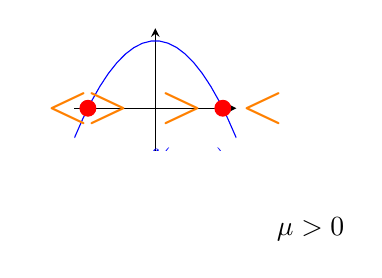
\begin{tikzpicture}
        \begin{axis}[
                width=0.3\textwidth,
                axis lines=middle,
                axis equal,
                no markers,
                domain=-1.2:1.2,
                xtick=\empty,
                ytick=\empty]

            \addplot[blue, samples=20] {-x^2 + 1} node[below left] {$f(u,\mu)$};

            \coordinate (O1) at (axis cs: -1, 0);
            \coordinate (O2) at (axis cs: 1, 0);

            \coordinate (l1) at (axis cs: -1.3, 0);
            \coordinate (r1) at (axis cs: -0.7, 0);
            \coordinate (l2) at (axis cs: 1.6, 0);
            \coordinate (r2) at (axis cs: 0.4, 0);
        \end{axis}

        \node[orange, scale=2] at (l1) {$<$};
        \node[orange, scale=2] at (r1) {$>$};
        \node[orange, scale=2] at (l2) {$<$};
        \node[orange, scale=2] at (r2) {$>$};

        \draw[red, fill] (O1) circle (0.1);
        \draw[red, fill] (O2) circle (0.1);

        \node at (3, -1) {$\mu > 0$};
    \end{tikzpicture}


\end{center}

Which yields the bifurcation diagram:
\begin{center}
    % Left parabola
    \begin{tikzpicture}
        \begin{axis}[no markers,
                axis lines=middle,
                domain=-1.2:1.2,
                xtick=\empty,
                ytick=\empty,
                clip=false]
            \addplot[blue] ({x^2}, x);

            \addplot[dashed] ({-1}, x) node[above] {$\mu < 0$};
            \addplot[dashed] ({1}, x) node[above] {$\mu > 0$};

            \coordinate (u1) at (axis cs:1, -1);
            \coordinate (u2) at (axis cs:1, 1);
            \coordinate (o) at (axis cs:0, 0);
        \end{axis}
        \draw[red, fill] (u1) circle (0.1);
        \draw[red, fill] (u2) circle (0.1);
        \draw[red, fill] (o) circle  (0.1);

        \node[orange, scale=1.5] at (5.6, 0) {\rotatebox{180}{$\wedge$}};
        \node[orange, scale=1.5] at (5.6, 0.9) {$\wedge$};

        \node[orange, scale=1.5] at (5.6, 5.7) {$\wedge$};
        \node[orange, scale=1.5] at (5.6, 4.7) {\rotatebox{180}{$\wedge$}};

        \node[orange, scale=1.5] at (0, 4.7) {\rotatebox{180}{$\wedge$}};
        \node[orange, scale=1.5] at (0, 1.5) {\rotatebox{180}{$\wedge$}};

        \node at (3, -1) {(2): \quad $g'(0) = 0, g''(0) \neq 0$};
    \end{tikzpicture}

\end{center}


\subsection{Stability at the Equilibria}
If $u = u_*$ is an equilibrium of $\dot u = f(u, \mu)$ at $\mu = \mu_*$, then
\[\begin{cases}
        f_u(u_*, \mu_*) > 0 & \text{unstable}     \\
        f_u(u_*, \mu_*) < 0 & \text{stable}       \\
        f_u(u_*, \mu_*) = 0 & \text{undetermined}
    \end{cases}\]

We know that our equilibria occur at $(u, \mu) = (u, g(u))$. Hence, we must check the condition $f_u(u, g(u))$. The process is the same as before:

Take the Taylor Expansion:
\begin{align*}
    f(u, \mu)   & = f_{\mu}(0, 0) \mu + \frac{f_{uu}(0, 0)}{2} u^2 + O(\mu u + \mu^2 + u^3) \\
    f_u(u, \mu) & = f_{uu}(0, 0)u + O(\mu + u^2)                                            \\
\end{align*}

Taking $g(\mu) = -\frac{f_{uu}(0, 0)}{f_{\mu}(0, 0)}u^2 + O(u^3) = O(u^2)$, notice that evaluating $f_u(u, \mu)$ at $(u, \mu) = (u, g(u))$,
\[O(\mu + u^2) = O(g(u) + u^2) = O(u^2)\]
so
\[f_u(u, g(u)) = f_{uu}(0,0)u + O(u^2)\]

Hence, the equilibrium $u$ at $\mu = g(u)$ is
\begin{itemize}
    \item stable for $f_{uu}(0, 0) u < 0$
    \item unstable for $f_{uu}(0, 0) u > 0$
\end{itemize}

\end{document}

